% -*- root: ../../DAT2-A423_Project_Report.tex -*-
\section{Optimisation}
We have managed to implement several complex algorithms in our programme.
This was immediately visible if the JPEG-encoder was run with larger images (such as the 4K (3840x2160) resolution images that the camera in many smart phones output) or if long messages of several hundred bytes were embedded in the image.
Doing so took upwards of several minutes on slower computers, so some optimisation of the code was clearly a requirement.
This section will focus on how these optimisations were implemented.
\vspace*{12pt}

To see what kinds of optimisations were useful and where they were needed, it was necessary to objectively measure their worth.
The easiest way to do this, was by timing how long different parts of the code took to complete.
To show this, we created a Stopwatch object in JPEGImage, which allowed us to keep track of how many milliseconds something took.
In order to ensure that we could compare the timings from different runs, it was important to establish some base rules to follow.
We used the same image and message for every run.
The image is a 4K resolution jpg image of a landscape with a hot air balloon in it.
To ensure that we ran the method \lstinline|_padCoverImage|, we removed eight pixels from the right and bottom sides of the image, bringing the resolution to 3832x2152.
The message consisted of 640 bytes of the ASCII characters \textit{A-Z}.
This was equivalent to the length of four regular SMS messages end-to-end, and therefore constituted what we believed to be a message capable of containing enough information for most regular uses.

All runs were done on a \textit{Release} build, as there seemed to be significant overhead on a \textit{Debug} build.
Some basic optimisations such as moving the calculation of the upper-bound outside the declaration of for-loops had already been done at this point.
While being a very simple thing to do, this did have some visible results in a few areas.

We used a profiler to get a better understanding of which parts of the code took a substantial amount of time to run.
The following methods and procedures constituted around 90\% of the total time spent by our mostly unoptimised programme, when run with the aforementioned parameters:
\lstinline|_padCoverImage|, \lstinline|_splitToChannels|, \lstinline|_encodeAndQuantizeValues|, Adding edges to the graph, \lstinline|GetSwitches| and \lstinline|_huffmanEncoding|.
All numbers are averages based on ten consecutive runs, following a single "warm-up run", whose results were not saved.
This was done to get more stable timings, seeing as the first run always had slightly different times than the remaining.
It is quite possible that this was caused by the garbage collector, since it changes its behaviour depending on the patterns of code being run.
Therefore, running the programme once without saving the data allowed it to learn the memory allocation patterns of the code and react in the same way the next ten times it was run.
The warm-up run also allowed us to run the decoder to make sure that the message was being encoded properly in the image and that our optimisations had not changed the programme's output.
We completed a total of three rounds of optimisations, each further improving the performance of the programme.
The four different versions of the programme can be found in appendix \ref{app:E}.
The first runs and the control for our further tests are shown in table \ref{fig:0genoptimised}.

\vspace{12pt}
\begin{table}[H]
	\centering
	\caption{Unoptimised encoding for three different processors.}
	\label{fig:0genoptimised}
	\begin{tabular}{@{}llll@{}}
		\toprule
		Code segment            & \multicolumn{3}{c}{Processor}                                                                                                                                                                                                                                                    \\ \midrule
								& \begin{tabular}[c]{@{}l@{}}Intel\textsuperscript{\textregistered}\\ i5-4670K\end{tabular} & \begin{tabular}[c]{@{}l@{}}Intel\textsuperscript{\textregistered}\\ i7-4700HQ\end{tabular} & \begin{tabular}[c]{@{}l@{}}AMD\textsuperscript{\textregistered}\\ A6-3420M\end{tabular} \\ \midrule
		Image padding           & 6840 ms                                                                                   & 8060 ms                                                                                    & 39189 ms                                                                                \\
		Channel split           & 3081 ms                                                                                   & 3670 ms                                                                                    & 20775 ms                                                                                \\
		Encoding                & 4299 ms                                                                                   & 5304 ms                                                                                    & 28603 ms                                                                                \\
		Adding edges            & 525 ms                                                                                    & 626 ms                                                                                     & 4017 ms                                                                                 \\
		Get switches            & 1461 ms                                                                                   & 1764 ms                                                                                    & 10393 ms                                                                                \\
		Huffman                 & 642 ms                                                                                    & 761 ms                                                                                     & 3576 ms                                                                                 \\ \midrule
		\textbf{Total run time} & \textbf{17067 ms}                                                                         & \textbf{21393 ms}                                                                          & \textbf{108139 ms}                                                                      \\
		\textit{Time covered}   & \textit{98.7\%}                                                                           & \textit{94.4\%}                                                                            & \textit{99.0\%}                                                                         \\ \bottomrule
	\end{tabular}
\end{table}

\subsection{First Round of Optimisations}
It was quite obvious that \lstinline|_padCoverImage|, \lstinline|_splitToChannels| and \lstinline|_encodeAndQuantizeValues| were the most time-consuming.
The first thing we focused on was \lstinline|_padCoverImage|, simply because it took almost twice as long as the second most time-consuming method.
JPEG-encoding requires images with both a width and a height that is divisible by 16.
If an image does not fulfil this, the last pixel is copied up to 15 times in the direction needed.
Since the \lstinline|System.Drawing.Bitmap| class does not allow for resizing of images, we needed to copy the entire image before being able to pad its bottom and right side.
We did this by looping through every pixel and copying it to the new \lstinline|Bitmap|.
This was done in two nested for-loops that ran from zero the width and zero to the height respectively.
On the 3832x2152 image used, this amounted to 8,246,464 iterations.
Every iteration used the \lstinline|Bitmap| class' methods \lstinline|GetPixel| and \lstinline|SetPixel|.
It is very likely that there is more to the property than simply returning a value and therefore quite a bit of overhead.
More specifically the methods are both wrappers for native functions contained in \lstinline|GDI+|. 
These might very well have to check several things before being able to return the pixel.

Using the \lstinline|System.Drawing.Graphics| class as show in listing \ref{lst:copyBitmap} we were able to copy portions of \lstinline|Bitmap|s much more efficiently, \citep{MSDNBitmap} as can be seen in by the roughly 8000 \% decrease in time in table \ref{fig:1genoptimised}.


\begin{lstlisting}[firstnumber=684,label=lst:copyBitmap,caption={Copying a \lstinline|Bitmap| using the \lstinline|Graphics| class. \textbf{File:} first\textunderscore  round/JPEGImage.cs.}]
private static Bitmap _copyBitmap(Bitmap bitmapIn, int width, int height) {
    Bitmap bitmapOut = new Bitmap(width, height);
    Graphics g = Graphics.FromImage(bitmapOut);
    Rectangle rect = new Rectangle(0, 0, bitmapIn.Width, bitmapIn.Height);
    g.DrawImage(bitmapIn, rect, rect, GraphicsUnit.Pixel);
    g.Dispose();

    return bitmapOut;
}
\end{lstlisting}

Seeing this overhead on the \lstinline|Bitmap| class, made us suspect the same of the related \lstinline|System.Drawing.Color| class, which holds the data of a single pixel.
During \lstinline|_splitToChannels| we also looped through every pixel of the image and saved it in a temporary variable. 
From this we used the bytes \lstinline|R|, \lstinline|G| and \lstinline|B| three times each. 
In this round of optimisations we saved these values to temporary variables instead of getting them from the saved pixel each time they were needed.

This reduced the calls to the Pixel's getter, which had a positive impact on the overall performance of the method.
We also managed to get a slight increase in performance on the Huffman-encoding, by changing a loop in the \lstinline|BitList| to only run every eighth time a bit was added to the list.
This change can be seen in listings \ref{lst:originalCheckedAdd} and \ref{lst:newCheckedAdd}.

\begin{lstlisting}[firstnumber=85,label=lst:originalCheckedAdd, caption={Original \lstinline|CheckedAdd| in \lstinline|BitList|. Note the for-loop on line 93. It always runs. \textbf{File:} unoptimized/BitList.cs.}]
public void CheckedAdd(int val) {
    if (_addCounter % 8 == 0) {
        _latestEntries.SetAll(false);
    }
    _latestEntries[_addCounter % 8] = (val == 1);
    Add(val == 1);
    bool allOne = true;

    for (int i = 0; i < 8; i++) {
        if (!_latestEntries[i]) {
            allOne = false;
            break;
        }
    }

    if (allOne) {
        for (int i = 0; i < 8; i++) {
            Add(false);
        }
    }

    _addCounter++;
}
\end{lstlisting}

\begin{lstlisting}[firstnumber=26,label=lst:newCheckedAdd, caption={Improved \lstinline|CheckedAdd| in \lstinline|BitList|. The for-loop only runs an eighth of the time. \textbf{File:} first\textunderscore  round/BitList.cs.}]
public void CheckedAdd(int val) {
    if (_addCounter % 8 == 0) {
        _latestEntries.SetAll(false);
    }
    _latestEntries[_addCounter % 8] = (val == 1);
    Add(val == 1);
    bool allOne = false;

    if (_addCounter % 8 == 7) {
        allOne = true;
        for (int i = 0; i < 8; i++) {
            if (!_latestEntries[i]) {
                allOne = false;
                break;
            }
        }
    }

    if (allOne) {
        for (int i = 0; i < 8; i++) {
            Add(false);
        }
    }

    _addCounter++;
}
\end{lstlisting}

\vspace{12pt}
\begin{table}[H]
	\centering
	\caption{First round of optimisations. Improved \lstinline|Bitmap| copying, fewer calls to the properties of \lstinline|Pixel| and an improved \lstinline|BitList|.}
	\label{fig:1genoptimised}
	\begin{tabular}{@{}lllllll@{}}
		\toprule
		Code segment            & \multicolumn{6}{c}{Processor}                                                                                                                                                                                                                                                                                                                                                                                                                                                                                                     \\ \midrule
								& \begin{tabular}[c]{@{}l@{}}Intel\textsuperscript{\textregistered}\\ i5-4670K\end{tabular} & \begin{tabular}[c]{@{}l@{}}Decrease \\ in time\textsuperscript{\textdagger}\end{tabular} & \begin{tabular}[c]{@{}l@{}}Intel\textsuperscript{\textregistered}\\ i7-4700HQ\end{tabular} & \begin{tabular}[c]{@{}l@{}}Decrease\\ in time\textsuperscript{\textdagger}\end{tabular} & \begin{tabular}[c]{@{}l@{}}AMD\textsuperscript{\textregistered}\\ A6-3420M\end{tabular} & \begin{tabular}[c]{@{}l@{}}Decrease\\ in time\textsuperscript{\textdagger}\end{tabular} \\ \midrule
		Image padding           & 88 ms                                                                                     & 7673\%                                                                         & 101 ms                                                                                     & 7861\%                                                                        & 533 ms                                                                                  & 7246\%                                                                        \\
		Channel split           & 2988 ms                                                                                   & 3\%                                                                            & 3786 ms                                                                                    & -3\%                                                                          & 19431 ms                                                                                & 7\%                                                                           \\
		Encoding                & 4317 ms                                                                                   & 0\%                                                                            & 5145 ms                                                                                    & 3\%                                                                           & 29396 ms 																				& -3\%                                                                          \\
		Adding edges            & 524 ms                                                                                    & 0\%                                                                            & 627 ms                                                                                     & 0\%                                                                           & 4054 ms                                                                                 & -1\%                                                                          \\
		Get switches            & 1460 ms                                                                                   & 0\%                                                                            & 1765 ms                                                                                    & 0\%                                                                           & 10990 ms                                                                                & 0\%                                                                           \\
		Huffman                 & 541 ms                                                                                    & 19\%                                                                           & 651 ms                                                                                     & 17\%                                                                          & 3111 ms                                                                                 & 15\%                                                                          \\ \midrule
		\textbf{Total run time} & \textbf{10134 ms}                                                                         & \textbf{68\%}                                                                  & \textbf{12328 ms}                                                                          & \textbf{74\%}                                                                 & \textbf{68588 ms}                                                                       & \textbf{58\%}                                                                 \\
		\textit{Time covered}   & \textit{97.9\%}                                                                           & \textit{}                                                                      & \textit{98.0\%}                                                                            &                                                                               & \textit{98.4\%}                                                                         & \textit{}                                                                     \\ \bottomrule
	\end{tabular}
	\begin{tablenotes}
		\footnotesize{\item \textdagger As compared to the respective timings of table \ref{fig:0genoptimised}.}
	\end{tablenotes}
\end{table}

\subsection{Second Round of Optimisations}
While there was a slight speed-up by not accessing the properties of the \lstinline|Pixel| as often, it did not do as much.
It was apparent that any use of \lstinline|GetPixel| was going to cause problems on larger images.
Using \lstinline|LockBits| we were able to use an \lstinline|IntPtr| to point at the data in memory. \citep{MSDNIntPtr}
The reason for doing this instead of using an actual pointer, is the fact that pointers in C\# requires the code they are used in to be wrapped in the \lstinline|unsafe| keyword. 
We could not be entirely sure of the implications of this on an Android device, since it can require a different privileges on different platforms.
Using this method to get the \lstinline|R|, \lstinline|G| and \lstinline|B| components of the source \lstinline|Bitmap| was beneficial to the programme's execution time.
In fact, it was almost eight times faster than the previously used method, as seen on figure \ref{fig:2genoptimised}.

Several changes to the two nested loops, which added edges to the graph, resulted in an improvement as to the Adding edges step as well as \lstinline|GetSwitches|.
The original algorithm (as shown in listing \ref{lst:oldEdgeAdding}) had complexity $\mathcal{O}(n^2)$, so longer message lengths could result in much longer running times for it.

\begin{lstlisting}[firstnumber=459,label=lst:oldEdgeAdding, caption={Original algorithm for adding edges to the graph. \textbf{File:} first\textunderscore  round/JPEGImage.cs.}]
int threshold = 5;
foreach (Vertex currentVertex in graph.Vertices) {
    foreach (Vertex otherVertex in graph.Vertices.Where(otherVertex => currentVertex != otherVertex)) {
        _addEdge(true, true, currentVertex, otherVertex, threshold, graph);
        _addEdge(true, false, currentVertex, otherVertex, threshold, graph);
        _addEdge(false, true, currentVertex, otherVertex, threshold, graph);
        _addEdge(false, false, currentVertex, otherVertex, threshold, graph);
    }
}
\end{lstlisting}

We made sure to only look at the vertices whose vertices did not already fit with the message.
With an M-value of four this meant that we would not have to check if we could add edges to around 25\% of the vertices.
We further reduced the overall amount of times the loops ran, by making sure that the inner loop only looked ahead in the list of vertices, which meant we only had to add each edge once.
Before this, we were adding every edge twice, with the start and end vertex flipped.
This meant that our list of edges was halved, which effectively reduced the running time of \lstinline|GetSwitches| to a fourth.
These changes can be seen in listing \ref{lst:newEdgeAdding}.

\begin{lstlisting}[firstnumber=449,label=lst:newEdgeAdding, caption={Improved algorithm for adding edges to the graph. \textbf{File:} second\textunderscore  round/JPEGImage.cs.}]
List<Vertex> toBeChanged = graph.Vertices.Where(x => (x.SampleValue1 + x.SampleValue2).Mod(x.Modulo) != x.Message).ToList();
int length = toBeChanged.Count;
int threshold = 5;
for (int i = 0; i < length; i++) {
    for (int j = i + 1; j < length; j++) {
        _addEdge(true, true, toBeChanged[i], toBeChanged[j], threshold, graph);
        _addEdge(true, false, toBeChanged[i], toBeChanged[j], threshold, graph);
        _addEdge(false, true, toBeChanged[i], toBeChanged[j], threshold, graph);
        _addEdge(false, false, toBeChanged[i], toBeChanged[j], threshold, graph);
    }
}
\end{lstlisting}

On a smaller note, we also changed the order in which the three checks that took place in \lstinline|_addEdge|.
Two of these check were more computationally demanding than the third.
By moving the least demanding check so it was the first one evaluated, it meant that the more demanding checks were not performed quite as often.
This allowed us to save quite a few operations on each iteration.
Furthermore, we added the calculated edge weights to the edges instead of having a property that calculated them every time.
This saved a few operations at a later time, when the edges were ordered by weight.
The two different versions of \lstinline|_addEdge| can be seen in listings \ref{lst:oldAddEdge} and \ref{lst:newAddEdge}.

\begin{lstlisting}[firstnumber=478,label=lst:oldAddEdge, caption={The original \lstinline|_addEdge| method. \textbf{File:} first\textunderscore  round/JPEGImage.cs.}]
private static void _addEdge(bool firstFirst, bool secondFirst, Vertex first, Vertex second, int threshold, Graph g) {
    if (((firstFirst ? first.SampleValue2 : first.SampleValue1) + (secondFirst ? second.SampleValue1 : second.SampleValue2)).Mod(first.Modulo) == first.Message) {
        if (((firstFirst ? first.SampleValue1 : first.SampleValue2) + (secondFirst ? second.SampleValue2 : second.SampleValue1)).Mod(second.Modulo) == second.Message) {
            Edge e = new Edge(first, second, firstFirst, secondFirst);
            if (e.Weight < threshold) {
                g.Edges.Add(e);
            }
        }
    }
}
\end{lstlisting}

\begin{lstlisting}[firstnumber=482,label=lst:newAddEdge, caption={The improved \lstinline|_addEdge| method. \textbf{File:} second\textunderscore  round/JPEGImage.cs.}]
private static void _addEdge(bool firstFirst, bool secondFirst, Vertex first, Vertex second, int threshold, Graph g) {
    int weight = Math.Abs((firstFirst ? first.SampleValue1 : first.SampleValue2) - (secondFirst ? second.SampleValue1 : second.SampleValue2));
    if (weight < threshold) {
        if (((firstFirst ? first.SampleValue2 : first.SampleValue1) + (secondFirst ? second.SampleValue1 : second.SampleValue2)).Mod(first.Modulo) == first.Message) {
            if (((firstFirst ? first.SampleValue1 : first.SampleValue2) + (secondFirst ? second.SampleValue2 : second.SampleValue1)).Mod(second.Modulo) == second.Message) {
                Edge e = new Edge(first, second, weight, firstFirst, secondFirst);
                g.Edges.Add(e);
            }
        }
    }
}
\end{lstlisting}

\begin{table}[H]
	\centering
    \caption{Second round of optimisations. Using a pointer to recieve \lstinline|Bitmap| data directly and improved edge adding logic.}
    \label{fig:2genoptimised}
	\begin{tabular}{@{}lllllll@{}}
		\toprule
		Code segment            & \multicolumn{6}{c}{Processor}                                                                                                                                                                                                                                                                                                                                                                                                                                                                                                     \\ \midrule
								& \begin{tabular}[c]{@{}l@{}}Intel\textsuperscript{\textregistered}\\ i5-4670K\end{tabular} & \begin{tabular}[c]{@{}l@{}}Decrease \\ in time\textsuperscript{\textdagger}\end{tabular} & \begin{tabular}[c]{@{}l@{}}Intel\textsuperscript{\textregistered}\\ i7-4700HQ\end{tabular} & \begin{tabular}[c]{@{}l@{}}Decrease\\ in time\textsuperscript{\textdagger}\end{tabular} & \begin{tabular}[c]{@{}l@{}}AMD\textsuperscript{\textregistered}\\ A6-3420M\end{tabular} & \begin{tabular}[c]{@{}l@{}}Decrease\\ in time\textsuperscript{\textdagger}\end{tabular} \\ \midrule
		Image padding           & 88 ms                                                                                     & 7673\%                                                                         & 97 ms                                                                                      & 8249\%                                                                        & 503 ms                                                                                  & 7687\%                                                                        \\
		Channel split           & 356 ms                                                                                    & 765\%                                                                          & 386 ms                                                                                     & 850\%                                                                         & 5096 ms                                                                                 & 308\%                                                                         \\
		Encoding                & 4341 ms                                                                                   & -1\%                                                                           & 4796 ms                                                                                    & 11\%                                                                          & 29812 ms                                                                                & -4\%                                                                          \\
		Adding edges            & 219 ms                                                                                    & 140\%                                                                          & 116 ms                                                                                     & 442\%                                                                         & 629 ms                                                                                  & 539\%                                                                         \\
		Get switches            & 661 ms                                                                                    & 121\%                                                                          & 289 ms                                                                                     & 511\%                                                                         & 2244                                                                                    & 388\%                                                                         \\
		Huffman                 & 524 ms                                                                                    & 23\%                                                                           & 610 ms                                                                                     & 25\%                                                                          & 3125 ms                                                                                 & 14\%                                                                          \\ \midrule
		\textbf{Total run time} & \textbf{6405 ms}                                                                          & \textbf{166\%}                                                                 & \textbf{6534 ms}                                                                           & \textbf{227\%}                                                                & \textbf{42444 ms}                                                                       & \textbf{155\%}                                                                \\
		\textit{Time covered}   & \textit{96.6\%}                                                                           & \textit{}                                                                      & \textit{96.3\%}                                                                            &                                                                               & \textit{97.6\%}                                                                         & \textit{}                                                                     \\ \bottomrule
	\end{tabular}
	\begin{tablenotes}
		\footnotesize{\item \textdagger As compared to the respective timings of table \ref{fig:0genoptimised}.}
	\end{tablenotes}
\end{table}

\subsection{Third Round of Optimisations}
The final optimisations we did, had the potential to make a large difference on some systems.
Taking advantage of the multi-core design of most modern processors, we made some of the intensive parts of our code run in parallel on multiple threads, which can utilise multi-core systems.
The effects of this can vary widely depending on the processor architecture and not all smart phones would be able to take advantage of it.
The ones that can, should be able to see a dramatic increase in performance of some parts of the code.

Running loops in parallel as we did, required seeing the code and its data dependencies in a different way than we usually do.
With the exception of loops, normally, code is run from the top to the bottom.
The data dependencies follow the same pattern.
When it comes to multi-threaded code though, this pattern changes, since the same lines of code can potentially be accessed by different threads at the same time.
This can lead to race-conditions, where the result of code can change depending on which thread gets to make changes first.
Data can potentially be overwritten, since the same parts of memory can be written to at the same time.
In a high-level language such as C\#, this would most likely cause a run-time exception instead.
An example of a parallelised for-loop can be seen in listing \ref{lst:parallelEdgeAdding}.

\begin{lstlisting}[firstnumber=677,label=lst:parallelEdgeAdding, caption={Parallelisation of the algorithm for adding edges to the graph. \textbf{File:} third\textunderscore  round/JPEGImage.cs.}]
List<Vertex> toBeChanged = graph.Vertices.Where(x => (x.SampleValue1 + x.SampleValue2).Mod(x.Modulo) != x.Message).ToList();
int length = toBeChanged.Count;
int threshold = 5;
Parallel.For(0, length, i => {
    for (int j = i + 1; j < length; j++) {
        _addEdge(true, true, toBeChanged[i], toBeChanged[j], threshold, graph);
        _addEdge(true, false, toBeChanged[i], toBeChanged[j], threshold, graph);
        _addEdge(false, true, toBeChanged[i], toBeChanged[j], threshold, graph);
        _addEdge(false, false, toBeChanged[i], toBeChanged[j], threshold, graph);
    }
});
\end{lstlisting}

\FloatBarrier

Because of these dangers, it is important that one manages any and all of these synchronisation issues properly.
It is not always possible to use the same data-structure as single-threaded code does, and since we implemented multi-threading after making the code single-threaded we were not able to convert all the code.
Specifically Huffman-encoding proved too cumbersome to efficiently multi-thread.
However, DCT-calculation, quantization, adding edges and splitting the image to YCbCr-channels were successfully rewritten to allow for the code to run in parallel on several cores with the same output.

By using the smallest data types capable of holding our data and properly unloading large unused variables, we effectively reduced peak memory usage from almost 400MB to around 100MB.
This improved the spacial locality of the data, which had the potential of leading to better utilisation of the different levels of caches, all in all leading to a better performing programme.

Since we knew that there was a certain overhead on function calls, we tried to force the compiler to in-line some of the most called functions we had. 
This did not seem to have an effect, so it is quite likely that the compiler already in-lined the functions we had tried it on.

\begin{table}[H]
	\centering
    \caption{Third and last round of optimisations. Memory optimisations and multi-threading of several methods.}
    \label{fig:3genoptimised}
	\begin{tabular}{@{}lllllll@{}}
		\toprule
		Code segment            & \multicolumn{6}{c}{Processor}                                                                                                                                                                                                                                                                                                                                                                                                                                                                                                     \\ \midrule
								& \begin{tabular}[c]{@{}l@{}}Intel\textsuperscript{\textregistered}\\ i5-4670K\end{tabular} & \begin{tabular}[c]{@{}l@{}}Decrease \\ in time\textsuperscript{\textdagger}\end{tabular} & \begin{tabular}[c]{@{}l@{}}Intel\textsuperscript{\textregistered}\\ i7-4700HQ\end{tabular} & \begin{tabular}[c]{@{}l@{}}Decrease\\ in time\textsuperscript{\textdagger}\end{tabular} & \begin{tabular}[c]{@{}l@{}}AMD\textsuperscript{\textregistered}\\ A6-3420M\end{tabular} & \begin{tabular}[c]{@{}l@{}}Decrease\\ in time\textsuperscript{\textdagger}\end{tabular} \\ \midrule
		Image padding           & 87 ms                                                                                     & 7762\%                                                                         & 98 ms                                                                                      & 8107\%                                                                        & 511 ms                                                                                  & 7576\%                                                                        \\
		Channel split           & 143 ms                                                                                    & 2057\%                                                                         & 122 ms                                                                                     & 2914\%                                                                        & 769 ms                                                                                  & 2600\%                                                                        \\
		Encoding                & 1788 ms                                                                                   & 140\%                                                                          & 2447 ms                                                                                    & 117\%                                                                         & 6948 ms                                                                                 & 312\%                                                                         \\
		Adding edges            & 48 ms                                                                                     & 993\%                                                                          & 53 ms                                                                                      & 1074\%                                                                        & 197 ms                                                                                  & 1943\%                                                                        \\
		Get switches            & 294 ms                                                                                    & 397\%                                                                          & 333 ms                                                                                     & 430\%                                                                         & 2286                                                                                    & 378\%                                                                         \\
		Huffman                 & 527 ms                                                                                    & 22\%                                                                           & 624 ms                                                                                     & 22\%                                                                          & 3025 ms                                                                                 & 18\%                                                                          \\ \midrule
		\textbf{Total run time} & \textbf{3103 ms}                                                                          & \textbf{450\%}                                                                 & \textbf{3916 ms}                                                                           & \textbf{446\%}                                                                & \textbf{14764 ms}                                                                       & \textbf{632\%}                                                                \\
		\textit{Time covered}   & \textit{93.0\%}                                                                           & \textit{}                                                                      & \textit{93.9\%}                                                                            &                                                                               & \textit{93.0\%}                                                                         & \textit{}                                                                     \\ \bottomrule
	\end{tabular}
	\begin{tablenotes}
		\footnotesize{\item \textdagger As compared to the respective timings of table \ref{fig:0genoptimised}.}
	\end{tablenotes}
\end{table}

\subsection{Final product}
After having done these steps to optimise our programme, we ended up with a product that performed well enough for us to try testing it with larger message to see what we were able to encode in files.
We wanted to know if the capacity of the cover image or the time it took to encode the data was going to be the bottleneck.

The application can be seen on figure \ref{fig:formApp}. To test the image quality, we embedded a 4KB message into a 1024x683px image. With a quality of 53\% 4KB was the upper limit of how much data we could encode, while with a quality of 100\%, the image could contain 19KB of data.

On an Intel{\textregistered} Core\textsuperscript{\texttrademark} i5-3317U processor it took around 20 minutes to encode a 4KB message, while a 1KB message took 20 seconds to be encoded in the same image. This tells us that the encoding time plays a much larger role than the capacity of the image.

\begin{figure}
	\centering
	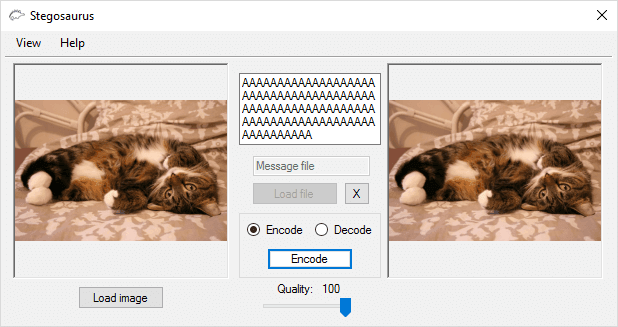
\includegraphics[width=.7\textwidth]{figures/formShown.png}
	\caption{Form}
	\label{fig:formApp}
\end{figure}

On figure \ref{fig:ResultEncoding} the results of the encoding are shown. There are no visible changes to the eye from figure \ref{fig:catHighMessage} to figure \ref{fig:catNoMessage}. This tells us that it is difficult for a person to tell the difference from the original image to the image with the encoded message. 

Likewise, there are no visible differences from figure \ref{fig:catJPEGMessage} to figure \ref{fig:catJPEGNoMessage}, which is the cover image encoded as JPEG at 53\% quality. The only differences from figure \ref{fig:catJPEGMessage} to the original cover image, is the overall lower quality from the JPEG compression, and not from the embedding of the message.

\begin{figure}[H]
    \centering
    \begin{subfigure}[b]{0.45\textwidth}
        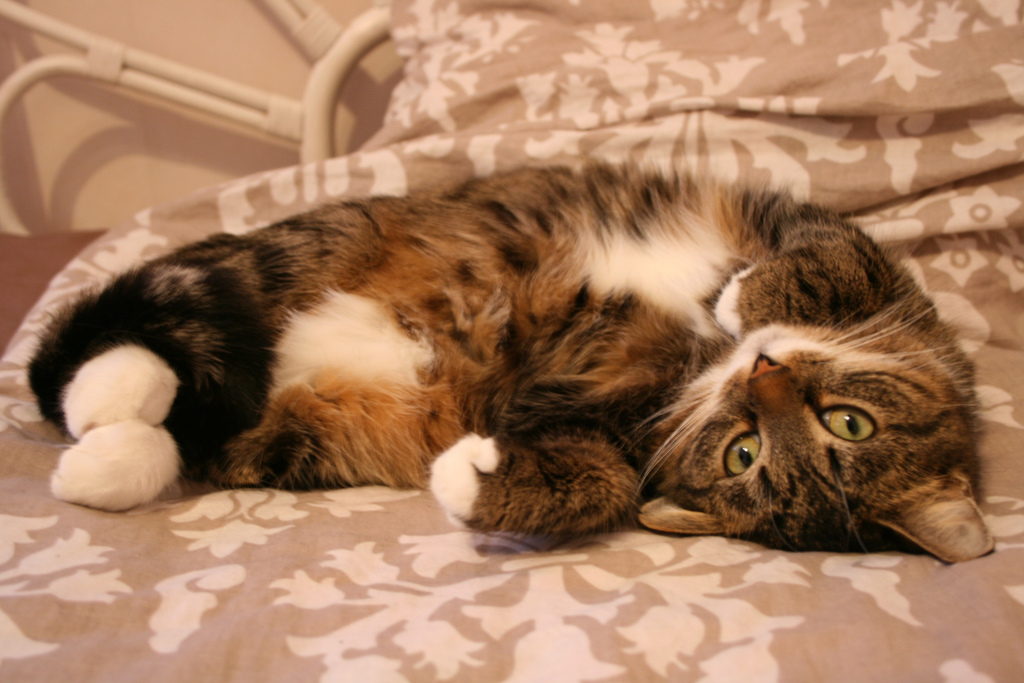
\includegraphics[width=\textwidth]{figures/catToTest.jpg}
		\caption{Cover image with no message encoded}
		\label{fig:catNoMessage}
    \end{subfigure}
    \begin{subfigure}[b]{0.45\textwidth}
        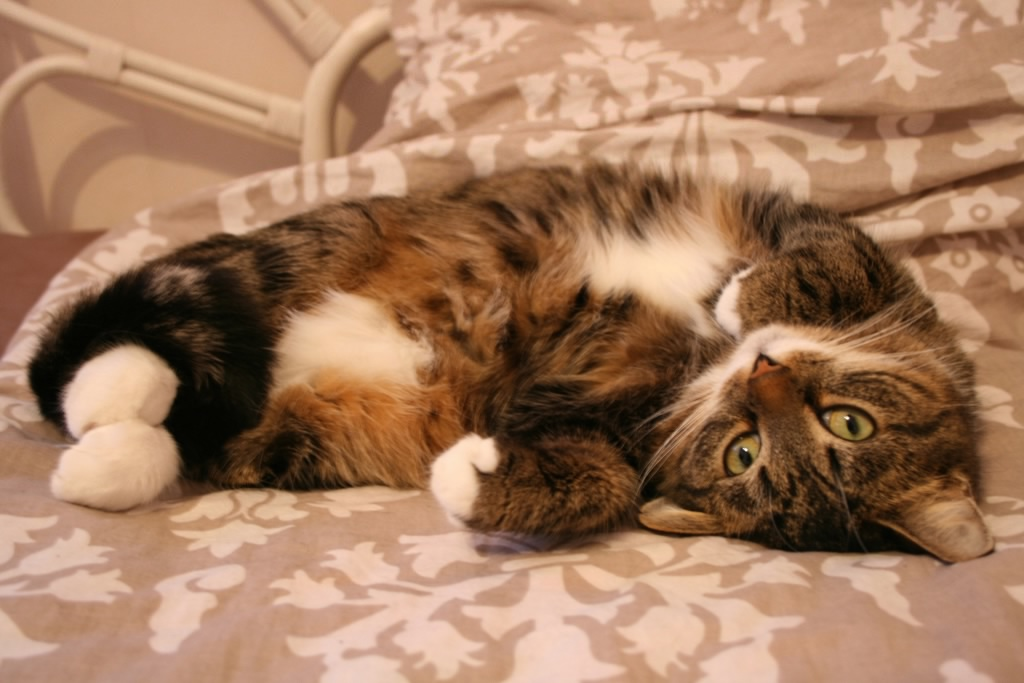
\includegraphics[width=\textwidth]{figures/catToTestHighMessage.jpeg}
		\caption{Encoded as JPEG with 4KB message with 100\% quality}
		\label{fig:catHighMessage}
    \end{subfigure}
    \begin{subfigure}[b]{0.45\textwidth}
        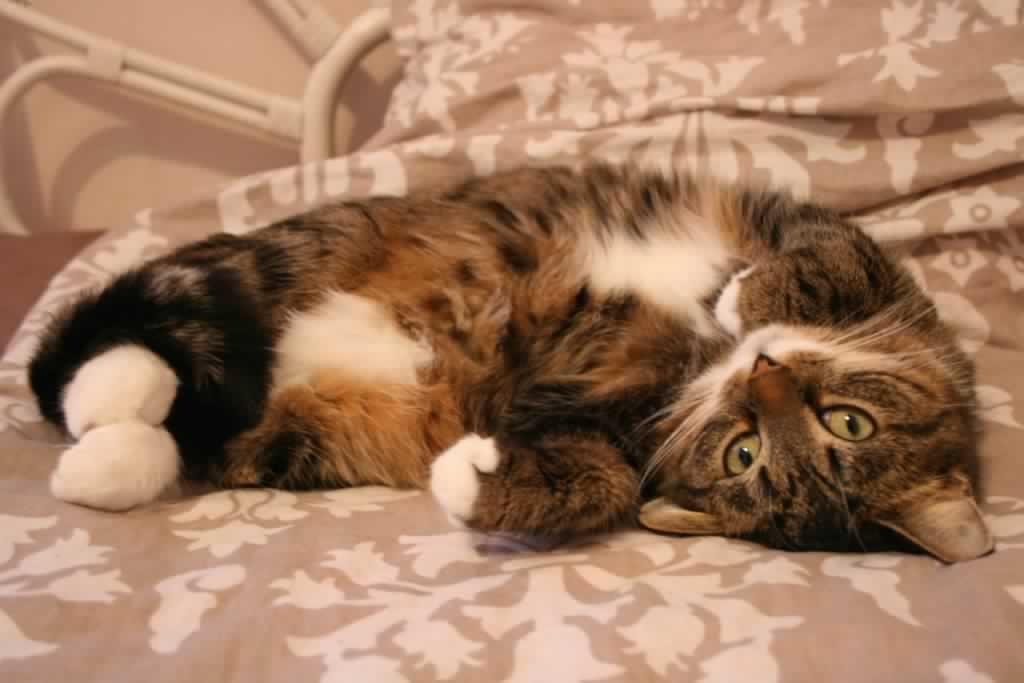
\includegraphics[width=\textwidth]{figures/catToTestNoMessage.jpeg}
		\caption{Encoded as JPEG with 53\% quality with no message}
		\label{fig:catJPEGNoMessage}
    \end{subfigure}
    \begin{subfigure}[b]{0.45\textwidth}
        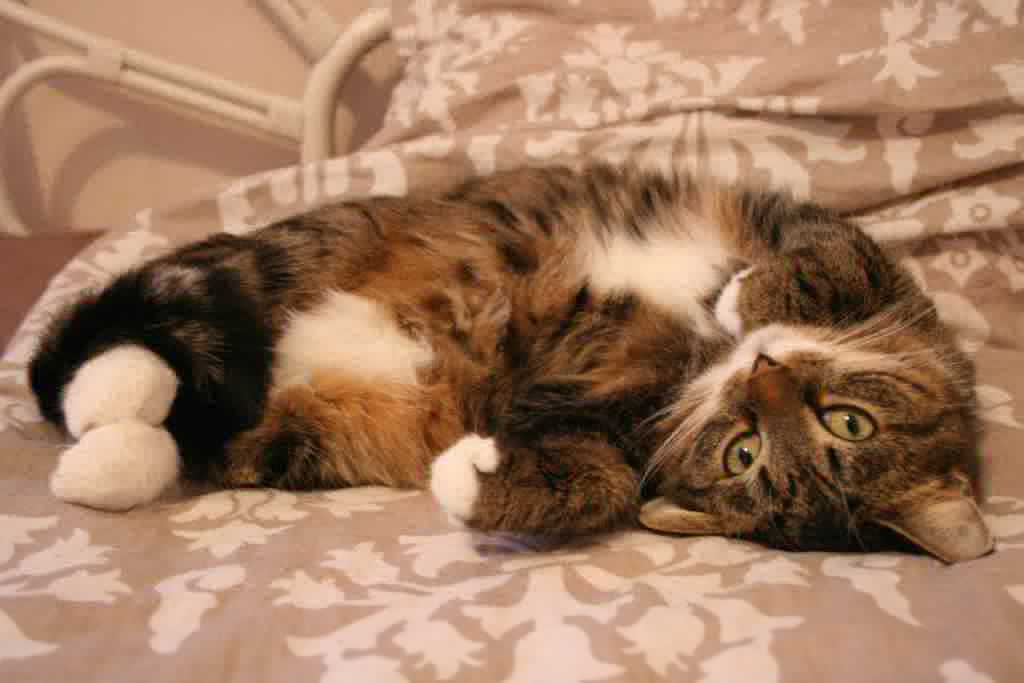
\includegraphics[width=\textwidth]{figures/catToTestWithMessage.jpeg}
		\caption{Encoded as JPEG with 53\% quality with 4KB message}
		\label{fig:catJPEGMessage}
    \end{subfigure}
    \caption{Encoding of the images \citep{FlickrImageCat}}
    \label{fig:ResultEncoding}
\end{figure}

Not being able to see the message with the naked eye is of course not enough, but it does tell us that the images are not changed greatly by embedding the message. In the next chapter, we will test the stego images by better means than simply looking at them. 